% !TeX root = ../main.tex
% Add the above to each chapter to make compiling the PDF easier in some editors.

\chapter{Evaluation}\label{chapter:evaluation}

\section{Testbed}
We now describe the testbed that we've used to evaluate and compare our streaming protocols. We perform multiple test runs for each streaming protocol, in which we first launch the client, establish a connection to the server and subscribe to the video stream. Once playback starts, we simulate various types of network patterns that are representative of real-world network conditions and collect relevant metrics. The network profiles used, which are taken from the Twitch's 2020 Grand Challenge on low-latency live streaming \parencite{ACMMMSys20}, are shown in \autoref{fig:bandwidth_profiles}.

\begin{figure}
    \centering
    
    % First row - Cascade profiles
    \begin{subfigure}[b]{0.3\textwidth}
        \centering
        \begin{tikzpicture}
            \begin{axis}[
                width=\textwidth,
                % xlabel={Time (s)},
                % ylabel={Bandwidth (Kbit/s)},
                ymin=0, ymax=1300, ytick distance=200,
                ymajorgrids=true,
                grid style=dashed,
                tick label style={font=\footnotesize},
                label style={font=\footnotesize},
            ]
            \addplot[red, const plot, thick, solid, mark=*] coordinates {
                (0,1200) (30,1200) (30,800) (60,800) (60,400) (90,400)
                (90,800) (120,800) (120,1200) (150,1200)
            };
            \end{axis}
        \end{tikzpicture}
        \caption{\footnotesize CASCADE}
    \end{subfigure}
    \begin{subfigure}[b]{0.3\textwidth}
        \centering
        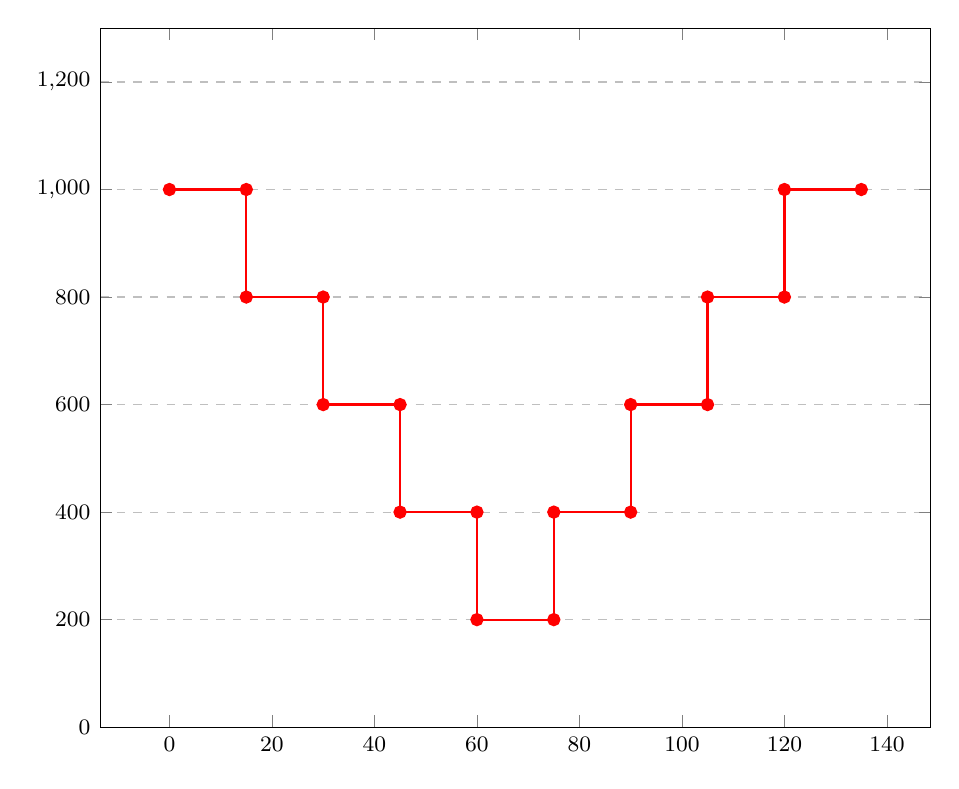
\begin{tikzpicture}
            \begin{axis}[
                width=\textwidth,
                % xlabel={Time (s)},
                % ylabel={Bandwidth (Kbit/s)},
                ymin=0, ymax=1300, ytick distance=200,
                ymajorgrids=true,
                grid style=dashed,
                tick label style={font=\footnotesize},
                label style={font=\footnotesize},
            ]
            \addplot[red, const plot, thick, solid, mark=*] coordinates {
                (0,1000) (15,1000) (15,800) (30,800) (30,600) (45,600) (45,400) (60,400)
                (60,200) (75,200) (75,400) (90,400) (90,600) (105,600) (105,800) (120,800)
                (120,1000) (135,1000)
            };
            \end{axis}
        \end{tikzpicture}
        \caption{\footnotesize INTRA\_CASCADE}
    \end{subfigure} 

    \vspace{1em}
    
    % Second row - Other profiles
    \begin{subfigure}[b]{0.3\textwidth}
        \centering
        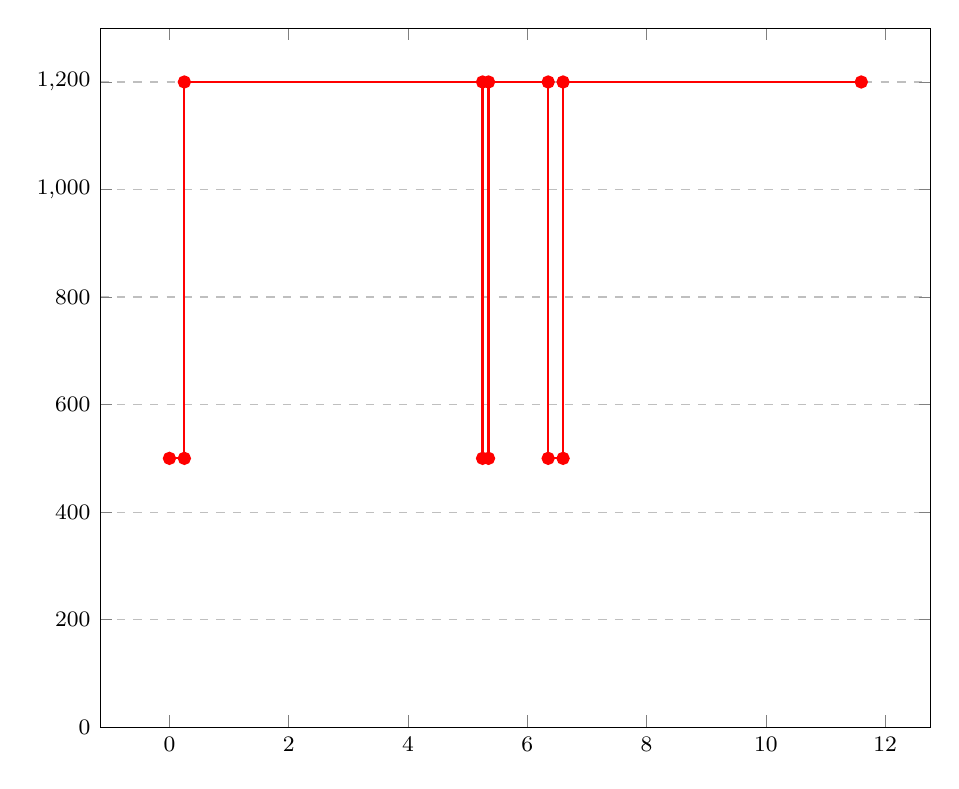
\begin{tikzpicture}
            \begin{axis}[
                width=\textwidth,
                % xlabel={Time (s)},
                % ylabel={Bandwidth (Kbit/s)},
                ymin=0, ymax=1300, ytick distance=200,
                ymajorgrids=true,
                grid style=dashed,
                tick label style={font=\footnotesize},
                label style={font=\footnotesize},
            ]
            \addplot[red, const plot, thick, solid, mark=*] coordinates {
                (0,500) (0.25,500) (0.25,1200) (5.25,1200) (5.25,500) (5.35,500)
                (5.35,1200) (6.35,1200) (6.35,500) (6.6,500) (6.6,1200) (11.6,1200)
            };
            \end{axis}
        \end{tikzpicture}
        \caption{\footnotesize FAST\_JITTERS}
    \end{subfigure}
    \begin{subfigure}[b]{0.3\textwidth}
        \centering
        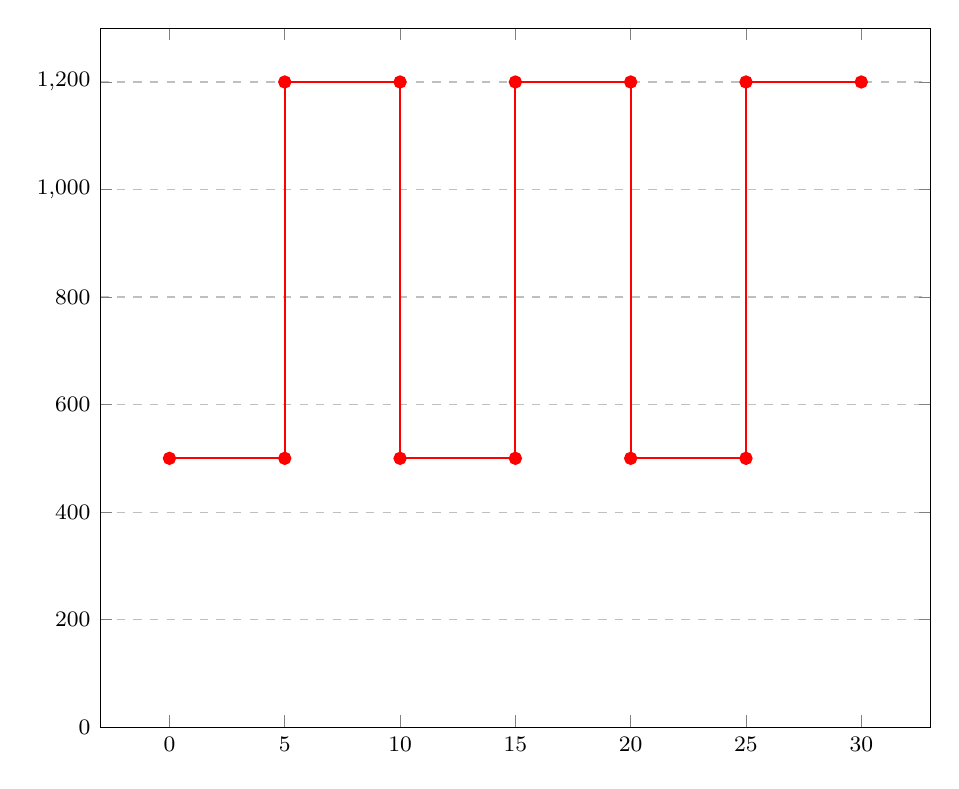
\begin{tikzpicture}
            \begin{axis}[
                width=\textwidth,
                % xlabel={Time (s)},
                % ylabel={Bandwidth (Kbit/s)},
                ymin=0, ymax=1300, ytick distance=200,
                ymajorgrids=true,
                grid style=dashed,
                tick label style={font=\footnotesize},
                label style={font=\footnotesize},
            ]
            \addplot[red, const plot, thick, solid, mark=*] coordinates {
                (0,500) (5,500) (5,1200) (10,1200) (10,500) (15,500) (15,1200) (20,1200)
                (20,500) (25,500) (25,1200) (30,1200)
            };
            \end{axis}
        \end{tikzpicture}
        \caption{\footnotesize SLOW\_JITTERS}
    \end{subfigure}
    \begin{subfigure}[b]{0.3\textwidth}
        \centering
        \begin{tikzpicture}
            \begin{axis}[
                width=\textwidth,
                % xlabel={Time (s)},
                % ylabel={Bandwidth (Kbit/s)},
                ymin=0, ymax=1300, ytick distance=200,
                ymajorgrids=true,
                grid style=dashed,
                tick label style={font=\footnotesize},
                label style={font=\footnotesize},
            ]
            \addplot[red, const plot, thick, solid, mark=*] coordinates {
                (0,1200) (10,1200) (10,300) (20,300) (20,800) (30,800)
            };
            \end{axis}
        \end{tikzpicture}
        \caption{\footnotesize SPIKE}
    \end{subfigure}

    \vspace{1em}

    \caption{Bandwidth profiles - Bandwidth (Kbit/s) vs. time (s)}
    \label{fig:bandwidth_profiles}
\end{figure}

We use dummynet\footnote{\url{https://man.freebsd.org/cgi/man.cgi?dummynet}} to emulate a link with limited bandwidth between the origin server and the client. Dummynet is a traffic shaping tool that simulates queue size and bandwidth limitations, delays and packet loss, by intercepting traffic between the transport protocol layers \parencite{rizzoDummynetSimpleApproach1997}. % TODO: I can expand on how it works if i want
In order to simulate the bandwidth limits we use a dummynet \textit{pipe} and feed traffic from the client to the server and vice versa into the pipe using PF\footnote{\url{https://www.openbsd.org/faq/pf/}} (Packet Filter).

The client and origin server run on the same machine, and communicate through the loopback interface. The origin server listens for incoming QUIC connections on port 443. We use PF rules that filter traffic on the localhost address from port 443 to any port, which corresponds to traffic between the server and the client, and forward it to the dummynet pipe. The dummynet pipe is configured with a bandwidth limit that varies according to the network profile throughout the test run. We don't configure any other options of the dummynet pipe explicitly, so that their default values are used. Some options worth mentioning include the queue size, which is set to 50 slots or packets by default, and the delay which is zero if not configured explicitly.

For the source video stream, we use the the Big Buck Bunny\footnote{\url{https://peach.blender.org/}} video and read the input file at the native frame rate using the ffmpeg option \lstinline{-re} to simulate live streaming. The video frame rate is 24 frames per second. We also reencode the video stream with AVC/H.264 using a custom bitrate and GoP structure, and repackage it in MP4 fragments. We use the following ffmpeg options to achieve this:
\begin{itemize}
    \item \lstinline{-an}: discard the audio track.
    \item \lstinline{-c:v libx264 -b:v 600k -bufsize 200K}: reencode the video using a target bitrate of 600 Kbit/s and a buffer size of 200 Kbit/s. The libx264 encoder is used.
    \item \lstinline{-g:v 15 -keyint_min:v 15 -sc_threshold:v 0}: set the minimum and maximum GoP size to 15 frames, and disables scene change detection so that each GoP has exactly the same size. 
    \item \lstinline{-bf 3}: set the maximum number of consecutive B-frames to 3. Note that the encoder can use a lower number B-frames between two reference frames.
    % \item \lstinline{-x264-params b-pyramid=none}: disable the use of B-frame as references for other frames to prevent video artifacts. The decoder produces video artifacts when it doesn't have a frame's dependencies as we described in \autoref{section:reference_b_frames}.
    \item \lstinline{-f mp4 -movflags cmaf+frag_every_frame}: use \ac{CMAF} compatible fragmented MP4 as the output format and package each frame in a separate fragment.
\end{itemize}

In both the deprioritize B-frames, and skip old \acp{GoP} approaches we use a buffer size of 100 ms for the jitter buffer. Furthermore, in the deprioritize B-frames approach, the reorder buffer has a size of 100 ms, leading to a total buffer buffer size of 200 ms. It is also worth mentioning that the server uses the BBR congestion control algorithm.

\section{Metrics}
We measure the latency of the live stream to evaluate the performance of our streaming protocols in poor network conditions. In a real-world live streaming system, many components in the media streaming pipeline contribute to the end-to-end latency \parencite{bentalebOneSecondLatencyEvolution2023}. In our measurements, we only take into account the latency added by the delivery and consumption phases, since our work focuses on the media distribution phase of the pipeline. We measure latency, as the delay between the frame reaching the server and being rendered in the client.  

% TODO: maybe cite where you got this idea from (dash player or twitch challenge testbed)
We measure the latency for each frame as follows. The server includes the availability time, the time at which the frame became available in the server, in the header of the MoQ object's payload. In the client, we calculate the latency for a given frame when the frame is rendered as the difference between the availability time and the time at which the frame was rendered. Note that both the server and client use the same clock, since they run on the same machine, and therefore clock drift is not an issue.

We would like to note however, that latency is not a complete metric by itself. Other factors such as rebuffering events, and stream quality are also important in determining the viewer's \ac{QoE}. An interesting area for future work is to use a weighted combination of these factors such as the \ac{QoE} model proposed by \citeauthor{yinControlTheoreticApproachDynamic2015} in \parencite{yinControlTheoreticApproachDynamic2015} to evaluate our approaches.

\section{Measurements}
We now present our measurements. We first analyse the deprioritize B-frames approach and we present data for two sample runs
one for the profile 500 Kbit/s and one for the profile INTRA-CASCADE. Then we present data for a sample run of the skip old
GoPs approach. Finally, we show the average latency for all profiles. 

Deprioritizing B-frames results in lower latencies when the network bandwidth is a little below the video stream's
bitrate. \autoref{fig:deprioritizing_b_frames_500Kbit:latency} shows the latency over time for sample runs of baseline and
deprioritize B-frames. In these test runs, the bandwidth is limited to 500 Kbit/s, which is 100 Kbit/s below the
target bitrate that we specifed in ffmpeg. In the beginning of the test, the latency for both versions is similar,
until around 0:40, when they diverge with the latency for deprioritize B-frames increasing at a slower rate than
the latency for baseline. The gap between the two versions increases steadily. At the 1:30 mark, the latency for 
deprioritize B-frames is about 5 seconds lower than the latency for baseline.

\begin{figure}
    \centering
    \begin{tikzpicture}
    \begin{axis}[
    axis lines=left,
    ylabel=Latency (ms),
    legend style={at={(0.98,0.02)}, anchor=south east, draw=none},
    legend cell align=left,
    scaled ticks=false,
    ymin=0, ymax=25000,
    xtick distance=0.5, minor x tick num=1,
    x filter/.code={\pgfmathparse{#1/60}}, % Convert seconds to minutes
    xticklabel={ % Split into hours and minutes
        \pgfmathsetmacro\hours{floor(\tick)}%
        \pgfmathsetmacro\minutes{(\tick-\hours)*0.6}%
        % Use some trickery to get leading zeros
        \pgfmathprintnumber{\hours}:\pgfmathprintnumber[fixed, fixed zerofill, skip 0.=true, dec sep={}]{\minutes}%
    },
    ]
    
    \addplot+[only marks] table[meta=latencyMs] {data/sample_runs_gop15/500Kbit/baseline/latency_per_sec.dat};
    \addplot+[only marks] table[meta=latencyMs] {data/sample_runs_gop15/500Kbit/b_frames/latency_per_sec.dat};
    
    \legend{Baseline, Deprioritizing B-frames}
    
    \end{axis}
\end{tikzpicture}
    \caption{Sample run of deprioritizing B-frames for profile 500 Kbit/s - Latency}
    \label{fig:deprioritizing_b_frames_500Kbit:latency}
\end{figure}

\begin{figure}
    \centering
    \centering
\begin{tikzpicture}
    \begin{axis}[
    width=0.48\textwidth,
    area style,
    axis lines=left,
    ylabel=Bitrate received (Kbit/s),
    title=Baseline,
    legend columns=-1,
    legend to name=named,
    scaled ticks=false,
    ymin=0, ymax=800, ytick distance=200,
    xtick distance=0.5, minor x tick num=1,
    x filter/.code={\pgfmathparse{#1/60}}, % Convert seconds to minutes
    xticklabel={ % Split into hours and minutes
        \pgfmathsetmacro\hours{floor(\tick)}%
        \pgfmathsetmacro\minutes{(\tick-\hours)*0.6}%
        % Use some trickery to get leading zeros
        \pgfmathprintnumber{\hours}:\pgfmathprintnumber[fixed, fixed zerofill, skip 0.=true, dec sep={}]{\minutes}%
    },
    ]
        \addplot+[fill=blue!20, draw=blue!40] table[meta=bitrateReceivedKbit] {data/sample_runs_gop15/500Kbit/baseline/total_bitrate.dat} \closedcycle;
        \addplot+[fill=green!20, draw=green!40] table[meta=bitrateReceivedKbit] {data/sample_runs_gop15/500Kbit/baseline/I_frames_bitrate.dat} \closedcycle;
        \addplot+[fill=orange!20, draw=orange!40] table[meta=bitrateReceivedKbit] {data/sample_runs_gop15/500Kbit/baseline/P_frames_bitrate.dat} \closedcycle;
        \addplot+[fill=purple!20, draw=purple!40] table[meta=bitrateReceivedKbit] {data/sample_runs_gop15/500Kbit/baseline/B_frames_bitrate.dat} \closedcycle;
        \addplot[ultra thick, red, no marks] coordinates {
        (0, 9999)
        (0, 500)
        (120, 500)
        (120, 9999)
        };
        \legend{Total, I-frames, P-frames, B-frames}
    \end{axis}
\end{tikzpicture}
%
\begin{tikzpicture}
    \begin{axis}[
    width=0.48\textwidth,
    area style,
    axis lines=left,
    title=Deprioritizing B-frames,
    scaled ticks=false,
    ymin=0, ymax=800, ytick distance=200,
    xtick={0.5, 1, 1.5, 2, 2.5},
    x filter/.code={\pgfmathparse{#1/60}}, % Convert seconds to minutes
    xticklabel={ % Split into hours and minutes
        \pgfmathsetmacro\hours{floor(\tick)}%
        \pgfmathsetmacro\minutes{(\tick-\hours)*0.6}%
        % Use some trickery to get leading zeros
        \pgfmathprintnumber{\hours}:\pgfmathprintnumber[fixed, fixed zerofill, skip 0.=true, dec sep={}]{\minutes}%
    },
    ]
        \addplot+[fill=blue!20, draw=blue!40] table[meta=bitrateReceivedKbit] {data/sample_runs_gop15/500Kbit/b_frames/total_bitrate.dat} \closedcycle;
        \addplot+[fill=green!20, draw=green!40] table[meta=bitrateReceivedKbit] {data/sample_runs_gop15/500Kbit/b_frames/I_frames_bitrate.dat} \closedcycle;
        \addplot+[fill=orange!20, draw=orange!40] table[meta=bitrateReceivedKbit] {data/sample_runs_gop15/500Kbit/b_frames/P_frames_bitrate.dat} \closedcycle;
        \addplot+[fill=purple!20, draw=purple!40] table[meta=bitrateReceivedKbit] {data/sample_runs_gop15/500Kbit/b_frames/B_frames_bitrate.dat} \closedcycle;
        \addplot[ultra thick, red, no marks] coordinates {
        (0, 9999)
        (0, 500)
        (120, 500)
        (120, 9999)
        };
    \end{axis}
\end{tikzpicture}

\bigskip
\ref{named}
    \caption{Sample run of deprioritizing B-frames for profile 500 Kbit/s - Bitrate received}
    \label{fig:deprioritizing_b_frames_500Kbit:bitrate_received}
\end{figure}

Taking a look at the frames that the clients in both approaches receive over time explains why.
\autoref{fig:deprioritizing_b_frames_500Kbit:bitrate_received} shows the bitrate of frames that reached the client
by frame type. Around the 0:40 mark, the client in deprioritize B-frames stops receiving B-frames,
which indicates that at this point the server stopped transmitting them. Because the server is not transmitting any
B-frames, more bandwidth is left for the base layer. Between 1:25
and 1:35 for example, baseline receives around 200 Kbit/s of B-frames 200 Kbit/s of P-frames, while deprioritize
B-frames receives 0 Kbit/s of B-frames and 300 Kbit/s of P-frames, which is 100 Kbit/s more than baseline.
Consequently, with deprioritize B-frames new frames are sent to the client sooner than with baseline,
such that the latency increases slower.

However, deprioritizing B-frames alone does not perform much better than baseline when the network bandwidth drops significantly
below the stream's bitrate. The reason for this is that B-frames make up only a small portion of the stream's total bitrate
compared to I-, and P-frames. \autoref{fig:deprioritizing_b_frames_intra_cascade:latency} shows the latency over time for
sample runs of baseline and deprioritize B-frames for the profile INTRA-CASCADE. Both versions show similar latencies
from 0:00 to 1:30. At around 1:30, after the bandwidth increased from 400 Kbit/s to 600 Kbit/s, the latency
stops growing for deprioritize B-frames, while for baseline it keeps increasing until 1:45.


Once again, the bitrate received by the client explains this.
\autoref{fig:deprioritizing_b_frames_intra_cascade:bitrate_received} shows the bitrate received by the client.
At the 1:07 mark, the client in deprioritize B-frames client stops receiving B-frames, indicating that the server has stopped
transmitting them. From this point onwards, the server only transmits frames from the base layer to the client.
When the network bandwidth increases from 400 Kbit/s to 600 Kbit/s, the latency stops increasing for deprioritize B-frames,
because 600 Kbit/s is above the base layer's bitrate. % TODO: Add a graph with the total bitrate and the bitrate of the base layer over time (if the network is not congested) to demonstrate this
600 Kbit/s is not big enough to be greater than the base layers plus the B-frames, which the server in baseline is transmitting, and therefore the latency keeps increasing until the bandwidth increases to 800 Kbit/s at 1:45. 

\begin{figure}
    \centering
    \begin{tikzpicture}
    \begin{axis}[
    axis lines=left,
    ylabel=Latency (ms),
    legend style={
        at={(0.5,-0.11)},
        anchor=north, 
        draw=none,
        cells={anchor=west},
        legend columns=-1,
        /tikz/every even column/.append style={column sep=0.2cm},
    },
    legend cell align=left,
    scaled ticks=false,
    ymin=0, ymax=30000, ytickmin=5000,
    xtick distance=0.5, minor x tick num=1,
    % xtick={0, 0.5, 1, 1.5, 2, 2.5},
    x filter/.code={\pgfmathparse{#1/60}}, % Convert seconds to minutes
    xticklabel={ % Split into hours and minutes
        \pgfmathsetmacro\hours{floor(\tick)}%
        \pgfmathsetmacro\minutes{(\tick-\hours)*0.6}%
        % Use some trickery to get leading zeros
        \pgfmathprintnumber{\hours}:\pgfmathprintnumber[fixed, fixed zerofill, skip 0.=true, dec sep={}]{\minutes}%
    },
    ]
        
        \addplot+[only marks] table[meta=latencyMs] {data/sample_runs_gop15/intra_cascade/baseline/latency_per_sec.dat};
        \addplot+[only marks] table[meta=latencyMs] {data/sample_runs_gop15/intra_cascade/b_frames/latency_per_sec.dat};
        
        \legend{Baseline, Deprioritizing B-frames}
    \end{axis}
\end{tikzpicture}
    \caption{Sample run of deprioritizing B-frames for profile INTRA-CASCADE - Latency}
    \label{fig:deprioritizing_b_frames_intra_cascade:latency}
\end{figure}

\begin{figure}
    \centering
    \centering
\begin{tikzpicture}
    \begin{axis}[
    width=0.48\textwidth,
    area style,
    axis lines=left,
    ylabel=Bitrate received (Kbit/s),
    title=Baseline,
    legend columns=-1,
    legend to name=named,
    scaled ticks=false,
    ymin=0, ymax=1000, ytick distance=200, ytickmin=200,
    xtick distance=0.5, minor x tick num=1,
    x filter/.code={\pgfmathparse{#1/60}}, % Convert seconds to minutes
    xticklabel={ % Split into hours and minutes
        \pgfmathsetmacro\hours{floor(\tick)}%
        \pgfmathsetmacro\minutes{(\tick-\hours)*0.6}%
        % Use some trickery to get leading zeros
        \pgfmathprintnumber{\hours}:\pgfmathprintnumber[fixed, fixed zerofill, skip 0.=true, dec sep={}]{\minutes}%
    },
    ]
        \addplot+[fill=blue!20, draw=blue!40] table[meta=bitrateReceivedKbit] {data/sample_runs_gop15/intra_cascade/baseline/total_bitrate.dat} \closedcycle;
        \addplot+[fill=green!20, draw=green!40] table[meta=bitrateReceivedKbit] {data/sample_runs_gop15/intra_cascade/baseline/I_frames_bitrate.dat} \closedcycle;
        \addplot+[fill=orange!20, draw=orange!40] table[meta=bitrateReceivedKbit] {data/sample_runs_gop15/intra_cascade/baseline/P_frames_bitrate.dat} \closedcycle;
        \addplot+[fill=purple!20, draw=purple!40] table[meta=bitrateReceivedKbit] {data/sample_runs_gop15/intra_cascade/baseline/B_frames_bitrate.dat} \closedcycle;
        \addplot[ultra thick, red, no marks] coordinates {
        (0, 1000)
        (15, 1000)
        (15, 800)
        (30, 800)
        (30, 600)
        (45, 600)
        (45, 400)
        (60, 400)
        (60, 200)
        (75, 200)
        (75, 400)
        (90, 400)
        (90, 600)
        (105, 600)
        (105, 800)
        (120, 800)
        (120, 1000)
        (135, 1000)
        };
        \legend{Total, I-frames, P-frames, B-frames}
    \end{axis}
\end{tikzpicture}
%
\begin{tikzpicture}
    \begin{axis}[
    width=0.48\textwidth,
    area style,
    axis lines=left,
    title=Deprioritizing B-frames,
    scaled ticks=false,
    ymin=0, ymax=1000, ytick distance=200, ytickmin=200,
    xtick distance=0.5, minor x tick num=1,
    x filter/.code={\pgfmathparse{#1/60}}, % Convert seconds to minutes
    xticklabel={ % Split into hours and minutes
        \pgfmathsetmacro\hours{floor(\tick)}%
        \pgfmathsetmacro\minutes{(\tick-\hours)*0.6}%
        % Use some trickery to get leading zeros
        \pgfmathprintnumber{\hours}:\pgfmathprintnumber[fixed, fixed zerofill, skip 0.=true, dec sep={}]{\minutes}%
    },
    ]
        \addplot+[fill=blue!20, draw=blue!40] table[meta=bitrateReceivedKbit] {data/sample_runs_gop15/intra_cascade/b_frames/total_bitrate.dat} \closedcycle;
        \addplot+[fill=green!20, draw=green!40] table[meta=bitrateReceivedKbit] {data/sample_runs_gop15/intra_cascade/b_frames/I_frames_bitrate.dat} \closedcycle;
        \addplot+[fill=orange!20, draw=orange!40] table[meta=bitrateReceivedKbit] {data/sample_runs_gop15/intra_cascade/b_frames/P_frames_bitrate.dat} \closedcycle;
        \addplot+[fill=purple!20, draw=purple!40] table[meta=bitrateReceivedKbit] {data/sample_runs_gop15/intra_cascade/b_frames/B_frames_bitrate.dat} \closedcycle;
        \addplot[ultra thick, red, no marks] coordinates {
        (0, 1000)
        (15, 1000)
        (15, 800)
        (30, 800)
        (30, 600)
        (45, 600)
        (45, 400)
        (60, 400)
        (60, 200)
        (75, 200)
        (75, 400)
        (90, 400)
        (90, 600)
        (105, 600)
        (105, 800)
        (120, 800)
        (120, 1000)
        (135, 1000)
        };
    \end{axis}
\end{tikzpicture}

\bigskip
\ref{named}
    \caption{Sample run of deprioritizing B-frames for profile INTRA-CASCADE - Bitrate received}
    \label{fig:deprioritizing_b_frames_intra_cascade:bitrate_received}
\end{figure}

Most importantly, the latency does not ever decrease for either approach, even when the network bandwidth increases above
the stream's bitrate at 1:30 and 1:45 respectively. This is because, in the client, both baseline and deprioritize B-frames
play old video before playing new video and never skip any video segments. 

% After 1:45, even though the latencies are not too far apart, Deprioritizing B-frames has an advantage.
% The buffer of the client in deprioritizing B-frames is increasing faster, because the server is not transmitting
% B-frames. Therefore if the network bandwidth decreases again, deprioritizing B-frames will be able to handle it
% better by going more time without rebuffering.

Thus, the bottom line is that to ensure low latencies adapting the stream quality is not sufficient by itself. % TODO: how many seconds
% . Even if there was a way to divide the stream into base and enhancement layers, such that the enhancement layer
% made up a much bigger portion of the total stream's bitrate, % TOOD: hierarchical schemes   We must skip
% that wouldn't be enough. In the worst-case if the network throughput is zero temporarily, once the network recovers,
% the latency won't decrease.
We need to skip old media to handle the cases in which the network bandwidth decreases significantly.

Skipping old GoPs decreases latency considerably in all types of network conditions. \autoref{fig:skipping_old_gops_intra_cascade:latency} shows the latency over time for a sample run of skip old GoPs for the profile INTRA-CASCADE and the same sample run of baseline. In contrast to baseline, the latency doesn't increase indefinitely from 0:30 onwards. Instead the latency per frame fluctuates, with the average latency being around
1.5 seconds throughout the middle of the test. Additionally, the latency decreases back to its minimum at 1:45.

\autoref{fig:skipping_old_gops_intra_cascade:latency_with_i_frames} marks the I-frames in the latency graph. In general,
the latency for each frame increases monotonically until the next I-frame, and then decreases. The maximum latency is therefore bound by the size of the GoP. Smaller GoPs result in lower latencies.

This is because I-frames are always transmitted as soon as the encoder produces them. \autoref{fig:skipping_old_gops_intra_cascade:pts_received} plots the pts of each frame that the client received against the local test time. For skip old GoPs the frames pts grows, in general, at exactly the same rate as the local time. Note that, as previously explained, the latency grows between every I-frame, however these small increases in latency are not visible in the graph. % TODO: Expand on why this is important. Thus, the latency is constant in the big picture. 
In contrast, the rate at which the frames pts for baseline increases slowly decreases beginning at 0:45.

Note as well that in skip old GoPs the client does not receive any frames between 0:63 and 0:75. The reason for this
is that the network bandwidth during this period is so low that there is not enough bandwidth to transmit the I-frame
of the current GoP before the I-frame of the next GoP becomes available. The average size of I-frames throughout this
test was around 173.76 Kbit. At 200 Kbit/s the server would need $173.76 Kbit/s / 200 Kbit/s \approx 0,87 s$ to transmit one I-frame. Since the frame rate is 24 frames per second, and the GoP size is 15 frames, the encoder produces a new I-frame every $1/24 * 15 = 0.625$ seconds though. As a result the server starts transmitting
the next I-frame, which has a higher priority, before it has finished transmitting the current one. Hence, no frames are fully transmitted during this period. This is the most significant disadvantage of our priority scheme. During this period baseline actually performs better than skip old GoPs.

\begin{figure}
    \centering
    \begin{tikzpicture}
    \begin{axis}[
    name=plot1,
    axis lines=left,
    ylabel=Latency (ms),
    legend style={at={(0.05,0.95)}, anchor=north west, draw=none},
    legend cell align=left,
    scaled ticks=false,
    ymin=0, ymax=25000,
    ytick distance={5000}, extra y ticks={1000}, ytickmin=1000,
    xtick distance=0.5, minor x tick num=1,
    x filter/.code={\pgfmathparse{#1/60}}, % Convert seconds to minutes
    xticklabel={ % Split into hours and minutes
        \pgfmathsetmacro\hours{floor(\tick)}%
        \pgfmathsetmacro\minutes{(\tick-\hours)*0.6}%
        % Use some trickery to get leading zeros
        \pgfmathprintnumber{\hours}:\pgfmathprintnumber[fixed, fixed zerofill, skip 0.=true, dec sep={}]{\minutes}%
    },
    ]
    
    \addplot+[only marks] table[meta=latencyMs] {data/sample_runs_gop15/intra_cascade/baseline/latency_per_sec.dat};
    \addplot+[only marks, color=brown] table[meta=latencyMs] {data/sample_runs_gop15/intra_cascade/gops/latency_per_sec.dat};
    
    \legend{Baseline, Skipping old GoPs}
    
    \end{axis}
    % \begin{axis}[
    %     % axis y line*=right,
    %     width=12cm,
    %     height=8cm,
    %     axis y line=right,
    %     axis x line=none,
    %     ylabel=Bandwidth (Kbit/s),
    %     ymin=0, ymax=1000,
    %     ]
        
    %     \addplot[red, no marks] coordinates {
    %         (0, 1000)
    %         (15, 1000)
    %         (15, 800)
    %         (30, 800)
    %         (30, 600)
    %         (45, 600)
    %         (45, 400)
    %         (60, 400)
    %         (60, 200)
    %         (75, 200)
    %         (75, 400)
    %         (90, 400)
    %         (90, 600)
    %         (105, 600)
    %         (105, 800)
    %         (120, 800)
    %         (120, 1000)
    %         (135, 1000)
    %     };

    % \end{axis}

    % Add legend outside the graph
    % \node[below=10pt of plot1.south, anchor=north, inner sep=0] (legend) {
    %     \begin{tikzpicture}
    %         \begin{customlegend}[
    %             legend entries={Baseline,Skipping old GoPs,Bandwidth},
    %             legend style={draw=none, column sep=5pt}
    %         ]
    %             \csname pgfplots@addlegendimage\endcsname{blue}
    %             \csname pgfplots@addlegendimage\endcsname{brown}
    %             \csname pgfplots@addlegendimage\endcsname{red}
    %         \end{customlegend}
    %     \end{tikzpicture}
    % };
\end{tikzpicture}
    \caption{Sample run of skipping old GoPs for profile INTRA-CASCADE - Latency}
    \label{fig:skipping_old_gops_intra_cascade:latency}
\end{figure}

\begin{figure}
    \centering
    \begin{tikzpicture}
    \begin{axis}[
        width=\textwidth,
        axis lines=left,
        ylabel=Latency (ms),
        legend style={
            at={(0.05,0.95)},
            anchor=north west,
            draw=none,
            font=\small,
            cells={anchor=west}
        },
        legend cell align=left,
        scaled ticks=false,
        ytick distance={5000}, extra y ticks={1000}, ytickmin=1000,
        xmin=0.5, xmax=1.75,
        xtick distance=0.25,
        x filter/.code={\pgfmathparse{#1/60}}, % Convert seconds to minutes
        xticklabel={ % Split into hours and minutes
            \pgfmathsetmacro\hours{floor(\tick)}%
            \pgfmathsetmacro\minutes{(\tick-\hours)*0.6}%
            % Use some trickery to get leading zeros
            \pgfmathprintnumber{\hours}:\pgfmathprintnumber[fixed, fixed zerofill, skip 0.=true, dec sep={}]{\minutes}%
        },
        ]
        
        \addplot+[color=brown] table[meta=latencyMs] {data/sample_runs_gop15/intra_cascade/gops/latency_per_sec_all_samples.dat};
        \addplot+[color=red, only marks, mark size=1pt] table[meta=latencyMs] {data/sample_runs_gop15/intra_cascade/gops/latency_per_sec_I_frames.dat};

        % \legend{All frames, I-frames}
        
    \end{axis}
    \end{tikzpicture}
    \caption{Sample run of skipping old GoPs for profile INTRA-CASCADE - Latency with I-frames}
    \label{fig:skipping_old_gops_intra_cascade:latency_with_i_frames}
\end{figure}

\begin{figure}
    \centering
    \begin{tikzpicture}
    \begin{axis}[
        axis lines=left,
        ylabel=Frame pts (sec),
        legend style={at={(0.98,0.02)}, anchor=south east, draw=none},
        legend cell align=left,
        scaled ticks=false,
        xmin=0.5, xmax=1.75,
        xtick distance=0.25,
        x filter/.code={\pgfmathparse{#1/60}}, % Convert seconds to minutes
        xticklabel={ % Split into hours and minutes
            \pgfmathsetmacro\hours{floor(\tick)}%
            \pgfmathsetmacro\minutes{(\tick-\hours)*0.6}%
            % Use some trickery to get leading zeros
            \pgfmathprintnumber{\hours}:\pgfmathprintnumber[fixed, fixed zerofill, skip 0.=true, dec sep={}]{\minutes}%
        },
        ]
        
        \addplot+[only marks, mark size=1.5pt] table[meta=ptsMs] {data/sample_runs_gop15/intra_cascade/baseline/pts_received_per_sec.dat};
        \addplot+[only marks, color=brown, mark size=1.5pt] table[meta=ptsMs] {data/sample_runs_gop15/intra_cascade/gops/pts_received_per_sec.dat};
        
        % \legend{Baseline, Skipping old GoPs}
    
    \end{axis}
    \end{tikzpicture}
    \caption{Frames received pts}
    \label{fig:skipping_old_gops_intra_cascade:pts_received}
\end{figure}

We now present the results of each approach for the twitch profiles. \autoref{fig:avg_latency} shows the average latency for each of our versions. Skip old GoPs is a clear winner, consistently showing lower latencies for all profiles. The difference is specially noticable for the CASCADE and INTRA-CASCADE profiles. On the other hand, deprioritize B-frames performs almost the same as baseline for all profiles. % Although, deprioritize B-frames achieves lower latencies in specific network bandwidth patterns, as \autoref{fig:deprioritizing_b_frames_500Kbit:latency} shows, it does not The profiles proposed by the twitch challenge are not ideal for deprioritize B-frames. Although in very specific types of network conditions, deprioritize B-frames does perform better than baseline as \autoref{fig:deprioritizing_b_frames_500Kbit:latency} shows.

\begin{figure}
    \centering
    \begin{tikzpicture}
\begin{axis}[
    ybar,
    ylabel={Average latency (ms)},
    scaled y ticks=false,
    ymin=0,
    ytick={0, 1000, 2000, 5000, 10000, 15000},
    xtick=data,
    xticklabels={CASCADE, FAST-JITTERS, INTRA-CASCADE, SLOW-JITTERS, SPIKE},
    x tick label style={font=\small},
    x tick label style={rotate=45, anchor=east},
    symbolic x coords={CASCADE, FAST-JITTERS, INTRA-CASCADE, SLOW-JITTERS, SPIKE},
    legend style={
        anchor=north,
        at={(0.5,1.15)},
        draw=none,
        legend columns=-1,
        /tikz/every even column/.append style={column sep=0.2cm},
    },
]

\addplot table {data/avg_latency/baseline.dat};
\addplot table {data/avg_latency/b_frames.dat};
\addplot table {data/avg_latency/gops.dat};

\legend{Baseline, Deprioritizing B-frames, Skipping old GoPs}

\end{axis}
\end{tikzpicture}
    \caption{Average latency (all profiles)}
    \label{fig:avg_latency}
\end{figure}

\section{Qualitative evaluation}
Having presented the measurements, we now discuss additional factors that influence the viability of each approach, but are hard to measure. 

Against deprioritizing B-frames:
\begin{itemize}
    \item Introduces temporal artifacts.
    \item Requires an encoding configuration that slightly increases the minimum latency. Deprioritize B-frames requires the encoder to produce some B-frames and the degree to which the system is able to cope with unfavourable network conditions is proportional to the size of the enhancement layer and therefore the number of B-frames. However, B-frames reference future frames, and therefore the encoder cannot produce them until after the future frames, meaning that B-frames add latency.
    \item The server has to understand and parse the codec with which the samples are encoded with to extract the type and dependencies of each frame. This adds complexity and creates a dependency on the video codec.
\end{itemize}

Against skipping old GoPs:
\begin{itemize}
    \item Excessive "warping" -- suddenly snapping forward to catch up to the live edge, when the video pauses or lags behind -- leads to a poor QoE. It is particularly noticable when the network bandwidth is extremely low and these jumps are frequent.
\end{itemize}
